%!TEX TS-program = xelatex
\documentclass[xetex]{beamer}

\usefonttheme{professionalfonts}

\usepackage[UTF8]{ctex}
\usepackage{hyperref}
\usepackage{unicode-math}
\usepackage{amsmath, amssymb}
\usepackage{graphicx, wrapfig}
\usepackage{nopageno}
\usepackage{animate}

\usetheme[block=fill]{metropolis}

\setmathfont{XITS Math}

\renewcommand{\qedsymbol}{\ensuremath{\blacksquare}}
\renewcommand{\footnotesize}{\tiny}

\title{曲线和曲面积分 I}
\subtitle{一型曲线和曲面积分}
\author{数学分析MOOC小组}
\date{}

\begin{document}
    \frame{\maketitle}

    \section{第一型曲线积分}

    \begin{frame}
        \frametitle{定义}
    
        \begin{block}{第一型曲线积分}
            设$L$是空间可求长的曲线段,$f(x,y,z)$定义在$L$上。$L$的两端点为$A$,$B$。依次用分点$A=A_0, A_1, \cdots, A_n = B$将$L$分成$n$小段,每小段的弧长记为$\Delta s_i$,不妨将第$i$小段弧也记为$\Delta s_i$。任取$(\xi_i, \eta_i, \zeta_i)\in\Delta s_i$,作和式
            $$\sum_{i=1}^{n}f(\xi_i, \eta_i, \zeta_i)\Delta s_i$$
            若当$\displaystyle\lambda = \max_{1\leq i \leq n}\left\{\Delta s_i\right\} \to 0$时上述和式极限存在,则称此极限为$f(x,y,z)$在曲线$L$上的\alert{第一型曲线积分},记为
            $$\int_Lf(x,y,z)\, \textrm{d}s$$
        \end{block}
    
    \end{frame}

    \begin{frame}
        \frametitle{简而言之}
    
        $$\int_Lf(x,y,z)\, \textrm{d}s = \lim_{\lambda \to 0}\sum_{i=1}^{n}f(\xi_i, \eta_i, \zeta_i)\Delta s_i$$
    
    \end{frame}

    \begin{frame}
        \frametitle{图解}
        \begin{figure}[ht]
            \centering
            \animategraphics[loop, autoplay, width=.5\linewidth, timeline=img/Line_integral_of_scalar_field/Line_integral_of_scalar_field.txt]{10}{img/Line_integral_of_scalar_field/Line_integral_of_scalar_field-}{0}{60}
            \caption{动图理解第一型曲线积分\footnote[1]{\href{https://commons.wikimedia.org/wiki/File:Line_integral_of_scalar_field.gif}{本图由作者Lucas Vieira释出至公有领域}}}
            \label{fig:intcurve}
        \end{figure}
    
    \end{frame}

    \begin{frame}
        \frametitle{计算}
    
        设$L$是光滑曲线
        $$x=x(t), y=y(t), z=z(t), \alpha \leq t \leq \beta$$
        $f(x,y,z)$在$L$上连续,则$f(x,y,z)$在$L$上的第一型曲线积分存在,且
        \begin{align*}
            &\int_Lf(x,y,z)\, \textrm{d}s \\
            =&\int_\alpha^\beta f(x(t), y(t), z(t))\sqrt{{x^\prime}^2(t) + {y^\prime}^2(t) + {z^\prime}^2(t)}\, \textrm{d}t\\
        \end{align*}
    
    \end{frame}

    \begin{frame}
        \frametitle{其他推断}
    
        当只有函数$L: y=g(x), \alpha \leq x \leq \beta$的时候,前面的公式可以写作
        \begin{align*}
            &\int_Lf(x,y)\, \textrm{d}s \\
            =&\int_\alpha^\beta f(x, g(x))\sqrt{1 + {g^\prime}^2(x)}\, \textrm{d}x\\
        \end{align*}

        这种特殊情况也是经常出题的情况。
    
    \end{frame}

    \section{第一型曲面积分}

    \begin{frame}
        \frametitle{定义}
    
        \begin{block}{第一型曲面积分}
            设$S$是空间光滑曲面$z=z(x,y), (x,y)\in D$,$f(x,y,z)$是定义在$S$上的函数。对于$D$的任意分法$\Delta \sigma_i$,相应地得到$S$的分法$\Delta S_i(i=1,2,\cdots, n)$。任取$(\xi_i, \eta_i, \zeta_i)\in\Delta S_i$,记$\displaystyle\lambda = \max_{1\leq i \leq n}\left\{\Delta \sigma_i\text{的直径}\right\}$。若极限
            $$\lim_{\lambda \to 0}\sum_{i=1}^{n}f(\xi_i, \eta_i, \zeta_i)\Delta S_i$$
            存在,则称该极限值为$f(x,y,z)$在曲面$S$上的\alert{第一型曲面积分},记为
            $$\iint_Sf(x,y,z)\, \textrm{d}S$$
        \end{block}
    
    \end{frame}

    \begin{frame}
        \frametitle{图解}
    
        \begin{figure}[ht]
            \centering
            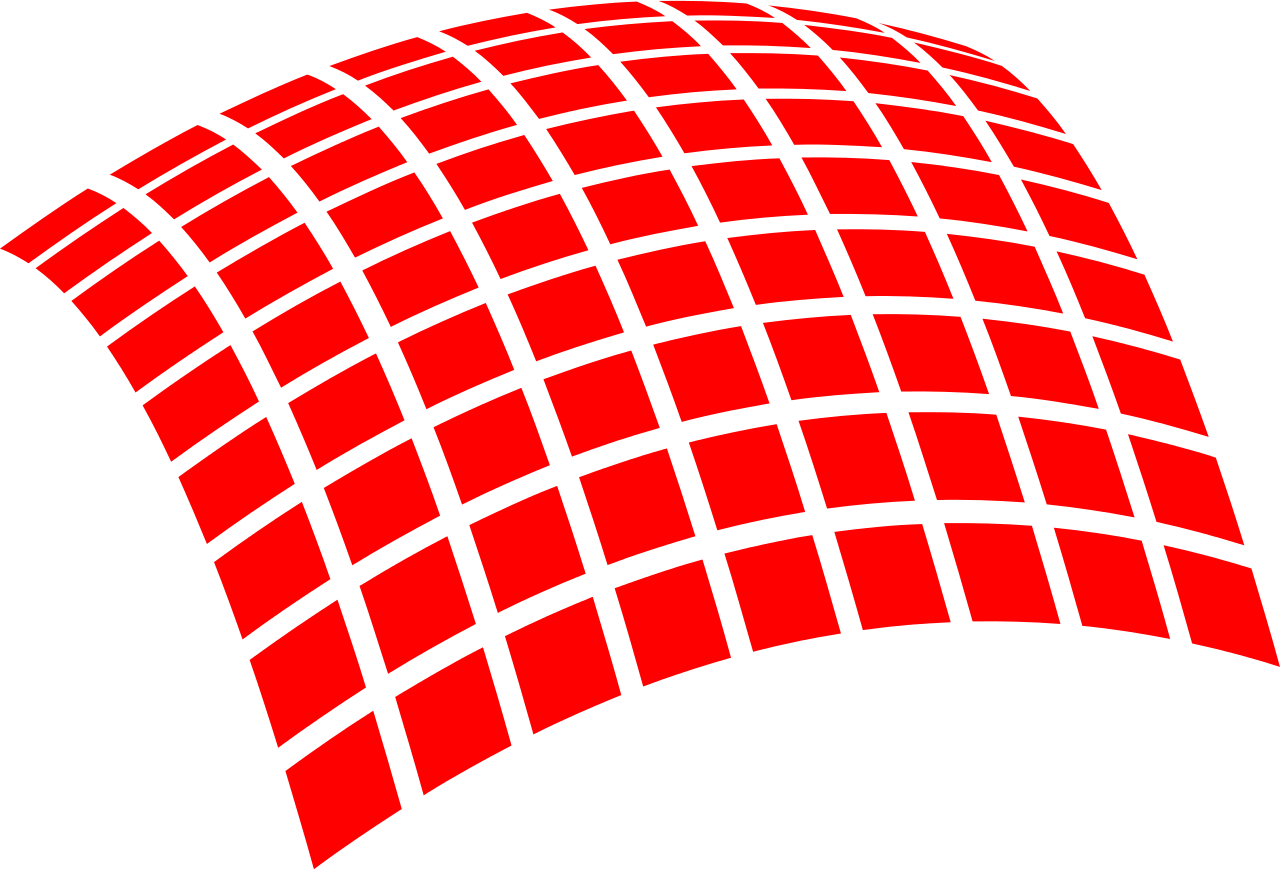
\includegraphics[width=.4\textwidth]{img/1280px-Surface_integral_illustration.svg.png}
            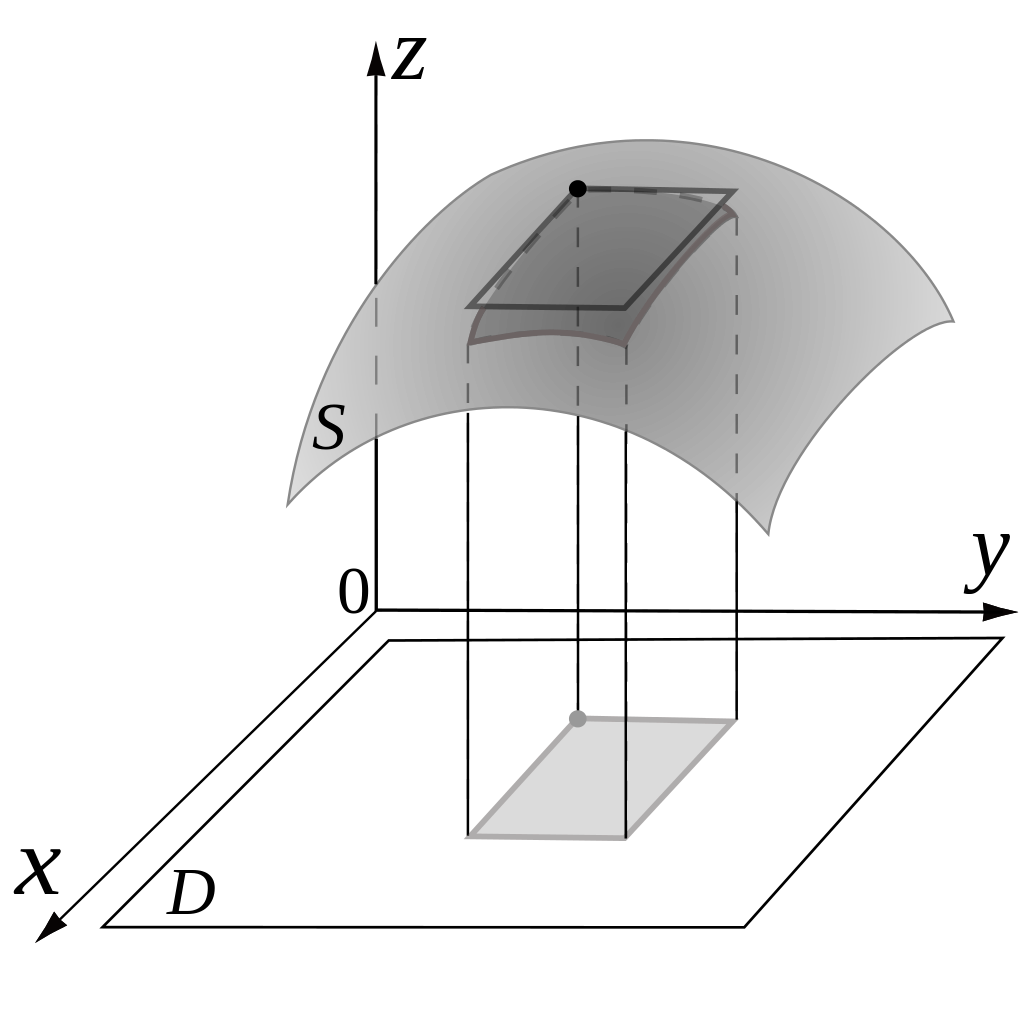
\includegraphics[width=.4\textwidth]{img/1034px-Surface_integral1.svg.png}
            \caption{将一个曲面细分为多个小块\footnote[1]{\href{https://commons.wikimedia.org/wiki/File:Surface_integral_illustration.svg}{左图由作者McMetrox以CC0 1.0协议公开}}\footnote[2]{\href{https://commons.wikimedia.org/wiki/File:Surface_integral1.svg}{右图由作者Cronholm144以CC-BY-SA 3.0协议公开}}}
            \label{fig:intplate}
        \end{figure}
    
    \end{frame}

    \begin{frame}
        \frametitle{计算}
    
        设$S: z=z(x,y), (x,y)\in D$是光滑曲面,$D$是有界闭区域,$f(x,y,z)$在$S$上连续,则$f(x,y,z)$在曲面$S$上的第一型曲面积分存在,且
        \begin{align*}
            &\iint_Sf(x,y,z)\, \textrm{d}S \\
            =&\iint_D f(x, y, z(x,y))\sqrt{z_x^2(x,y) + z_y^2(x,y)+1}\, \textrm{d}x\textrm{d}y\\
        \end{align*}
    
    \end{frame}

    \begin{frame}
        \frametitle{其他计算法}
    
        当光滑曲面由参数方程
        $$x=x(u,v), y=y(u,v), z=z(u,v), (u,v) \in D$$
        给出时,有
        \begin{align*}
            &\iint_Sf(x,y,z)\, \textrm{d}S \\
            =&\iint_D f(x(u,v), y(u,v), z(u,v))\sqrt{EG-F^2}\, \textrm{d}u\textrm{d}v\\
        \end{align*}
        其中$E=x_u^2+y_u^2+z_u^2, G=x_v^2+y_v^2+z_v^2, F=x_ux_v+y_uy_v+z_uz_v$

        这种题目不多,但是偏偏有的时候很好用。
    
    \end{frame}

    \section{例题}

    \begin{frame}
        \frametitle{曲线}
    
        计算$\displaystyle \int_L\left(x^2+y^2\right)\,\mathrm{d}s$,其中$L$为曲线$\displaystyle x=a\left(\cos t+t\sin t\right), y=a\left(\sin t-t\cos t\right), \left(0\leq t\leq 2\pi\right)$。
    
    \end{frame}

    \begin{frame}
        \frametitle{解}
    
        $$\mathrm{d}s=\sqrt{{x^\prime}^2+{y^\prime}^2}\mathrm{d}t=\sqrt{\left(at\cos t\right)^2+\left(at\sin t\right)^2}\mathrm{d}t=at\mathrm{d}t$$\pause
        $$\begin{aligned}
            \therefore \text{ 原式} &=\pause \int_{0}^{2\pi}a^2\left[\left(\cos t+t\sin t\right)^2+\left(\sin t-t\cos t\right)^2\right]at\,\mathrm{d}t \\\pause
            &= a^3\int_0^{2\pi}\left(t+t^3\right)\,\mathrm{d}t \\\pause
            &= a^3\left.\left(\frac{t^2}{2}+\frac{t^4}{4}\right)\right|_0^{2\pi} \\\pause
            &= 2\pi^2a^3\left(1+2\pi^2\right)
        \end{aligned}$$
        \qed
    
    \end{frame}

    \begin{frame}
        \frametitle{曲面}
    
        求$$\iint_\Sigma\frac{\mathrm{d}S}{x^2+y^2+z^2}$$其中$\Sigma$是界于平面$z=0$及$z=H$之间的圆柱面$x^2+y^2=R^2$。
    
    \end{frame}

    \begin{frame}
        \frametitle{解}
    
        柱面$\Sigma$按照对称面$xOz$分成两块,方程分别为\pause
        $$y=\sqrt{R^2-x^2}\text{ 和 }y=-\sqrt{R^2-x^2}$$\pause
        它们在$xOz$的投影均为$D_{xz}=\left\{\left.(z,x)\right|0\leq z \leq H, -R \leq x \leq R\right\}$\pause,且都有$$\sqrt{1+y_z^2+y_x^2}=\frac{R}{\sqrt{R^2-x^2}}$$\pause
        $$\begin{aligned}
            \therefore \text{ 原式} &=\pause 2\iint\frac{1}{R^2+z^2}\cdot\frac{1}{\sqrt{R^2-x^2}}\,\textrm{d}\sigma \\\pause
            &= 2\int_{-R}^R \frac{1}{\sqrt{R^2-x^2}}\,\mathrm{d}x\int_0^H\frac{1}{R^2+z^2}\,\mathrm{d}z\pause = 2\pi\arctan{\frac{H}{R}}
        \end{aligned}$$
        \qed
    
    \end{frame}

    \begin{frame}[standout]
    
        感谢

        \small{曲线和曲面积分 I · 终}
    
    \end{frame}
\end{document}
